\documentclass{beamer}
\usepackage[spanish]{babel}
\usepackage[utf8]{inputenc}
\usepackage{graphicx}
\graphicspath{ {./images/}}

\usetheme{Madrid}
\usecolortheme{default}

%------------------------------------------------------------
%This block of code defines the information to appear in the
%Title page
  \title[PC3 Estadística Aplicada] %optional
{Aplicación de tests no paramétricos}

\subtitle{
  Caso: Distribucion de notas de estudiantes de la academia
    Trilce en los ultimos 4 años
}

\author % (optional)
{
  Alvarez, Sandro \and Bautista, Walter \\ \and Burga, Ever \and
    Casanova, Italo \and  Cuyate, Brayan
}

\institute
{
  Facultad de Ingenieria Industrial y de Sistemas\\
  Estadística Aplicada - PC2\\
  \textbf{Universidad Nacional de Ingenieria}
}

\date
{Diciembre 2022}

% \logo{\includegraphics[height=1cm]{overleaf-logo}}

%End of title page configuration block
%------------------------------------------------------------

%------------------------------------------------------------
%The next block of commands puts the table of contents at the
%beginning of each section and highlights the current section:

% \AtBeginSection[]
% {
%   \begin{frame}
%     \frametitle{Tabla de Contenido}
%     \tableofcontents[currentsection]
%   \end{frame}
% }
% %------------------------------------------------------------


\begin{document}

%The next statement creates the title page.
\frame{\titlepage}

-----------------------------------------
\section{Objetivos}

%---------------------------------------------------------
\begin{frame}

\frametitle{Objetivos del trabajo}

\begin{alertblock}{General}
  Determinar si el ciclo de repaso ha sido útil para los postulantes a la
  Universidad Nacional de Ingenieria en la academia Trilce tomando en cuenta
  sus sedes y el efecto de la pandemia.
\end{alertblock}
\end{frame}


%---------------------------------------------------------
\section{Metodología y Resultados}

\begin{frame}
    \frametitle{Test de Kruskal-Wallis}
    % import image with a description
    La distribución de las notas de los estudiantes de la academia Trilce
    de acuerdo a sede es la siguiente: 
    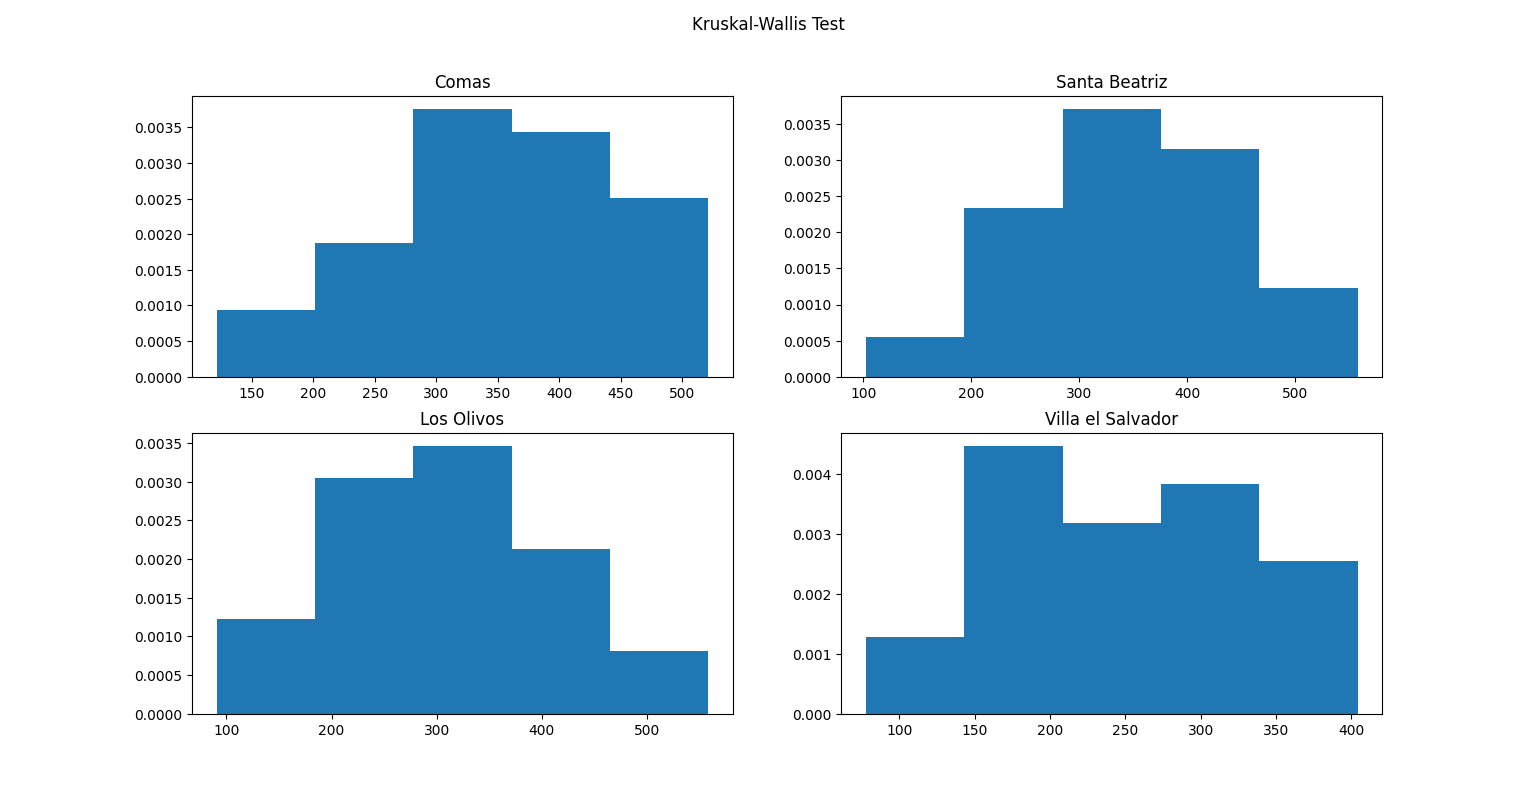
\includegraphics[width=1\textwidth]{cap/images/kruskal.png}
\end{frame}

\begin{frame}
    \frametitle{Test de Kruskal-Wallis}
    % import image with a description
    Con un gráfico de cajas se puede observar que la distribución de 
    Villa el Salvador tiene una mediana muestral que es distinta a las demás. 
    \centering
    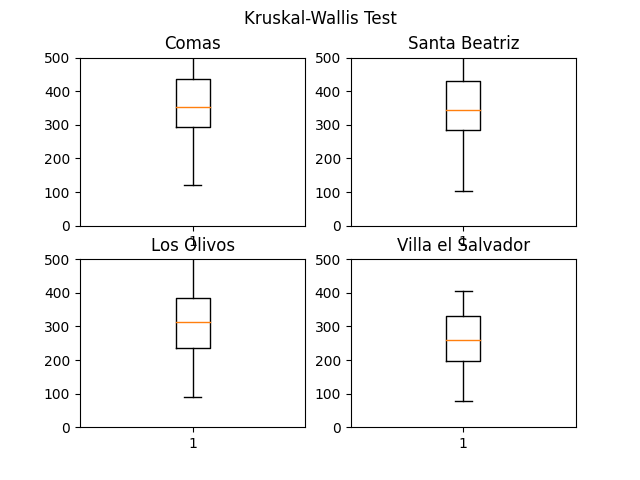
\includegraphics[width=0.8\textwidth]{cap/images/kruskal_boxplot.png}
\end{frame}

\begin{frame}
    \frametitle{Test de Kruskal-Wallis}
    % import image with a description
    \begin{itemize}
        \item Sea la hipótesis nula $H_0$ es que las distribuciones de las notas de los estudiantes de la academia Trilce de acuerdo a sede son iguales.
        \item La hipótesis alternativa $H_1$ es que al menos una de las distribuciones es distinta.
    \end{itemize}
    \begin{itemize}
        \item La prueba de Kruskal-Wallis arroja los siguientes resulados:
        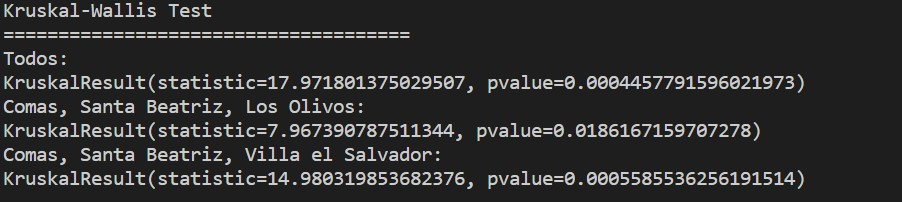
\includegraphics[width=0.8\textwidth]{cap/images/resultados_kruskal.jpg}
        \item Se rechaza $H_0$ y se concluye que al menos alguna distribución de notas de los estudiantes de la academia Trilce de acuerdo a sede difiere con un nivel de significancia del 5\%
    \end{itemize}
\end{frame}

\begin{frame}
    \frametitle{Test de Kruskal-Wallis}
    % import image with a description
    Al comparar las cuatro distribuciones el p-value es 0.000445. 
    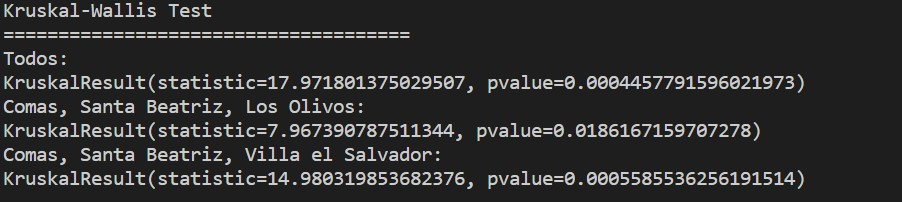
\includegraphics[width=0.8\textwidth]{cap/images/resultados_kruskal.jpg}
    
    Sin embargo, un detalle que resalta es que al excluir la distribución de Villa el Salvador, el p-value es 0.0186.
    Este valor sería significativo para un nivel de confianza del 1\% y señala una posible 
    diferencia que consideramos que es susceptible de futura investigación.
    
\end{frame}

\begin{frame}
    \frametitle{Prueba de aleatoriedad de rachas}
    Se realiza una prueba de rachas para determinar si los
    rankings de estudiantes de acuerdo a género son aleatorios
    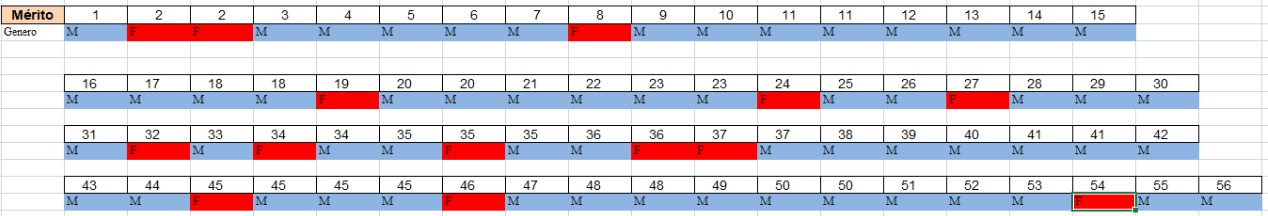
\includegraphics[width=1\textwidth]{cap/images/rachas/rachas_resultados.jpg}
\end{frame}

\begin{frame}
    \frametitle{Prueba de aleatoriedad de rachas}
    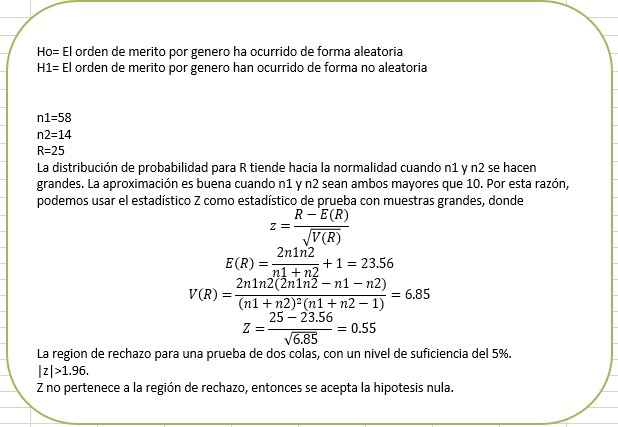
\includegraphics[width=1\textwidth]{cap/images/rachas/rachas_explicacion.jpg}
\end{frame}

\begin{frame}
    \frametitle{Test U de Mann-Whitney}
    % import image with a description
    Se ha comparado los resultados pre-pandemia y post-pandemia de los estudiantes de la academia Trilce.
    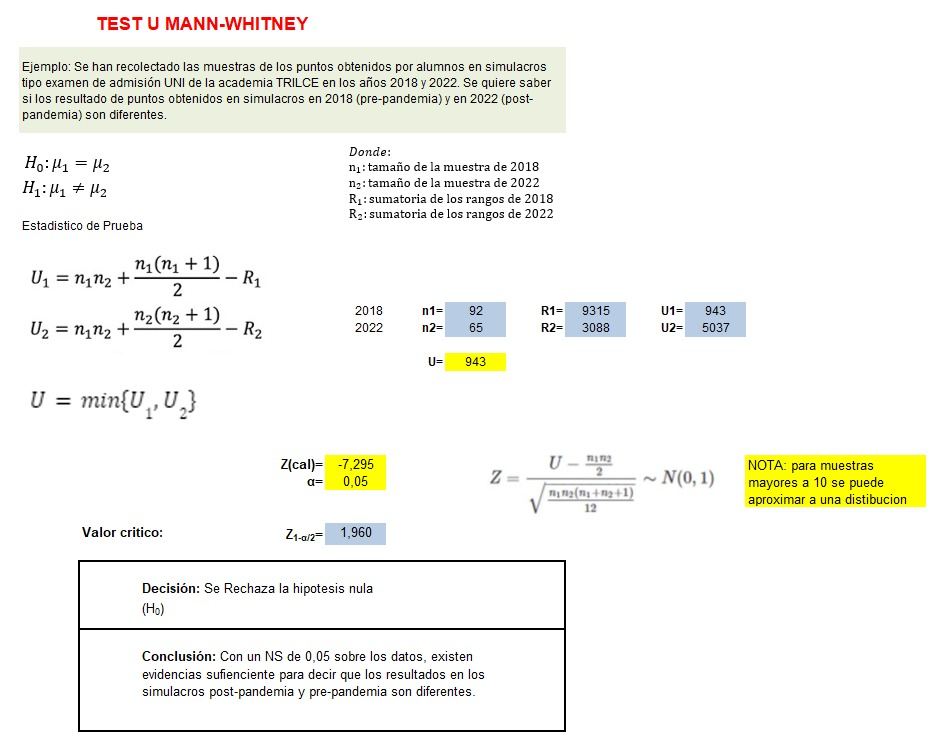
\includegraphics[width=0.8\textwidth]{cap/images/u_test/u_test.jpg}
\end{frame}


\begin{frame}
    \frametitle{Prueba de signos}
    Se realiza una prueba de signos para evaluar el desempeño de los estudiantes
    post-repaso.
    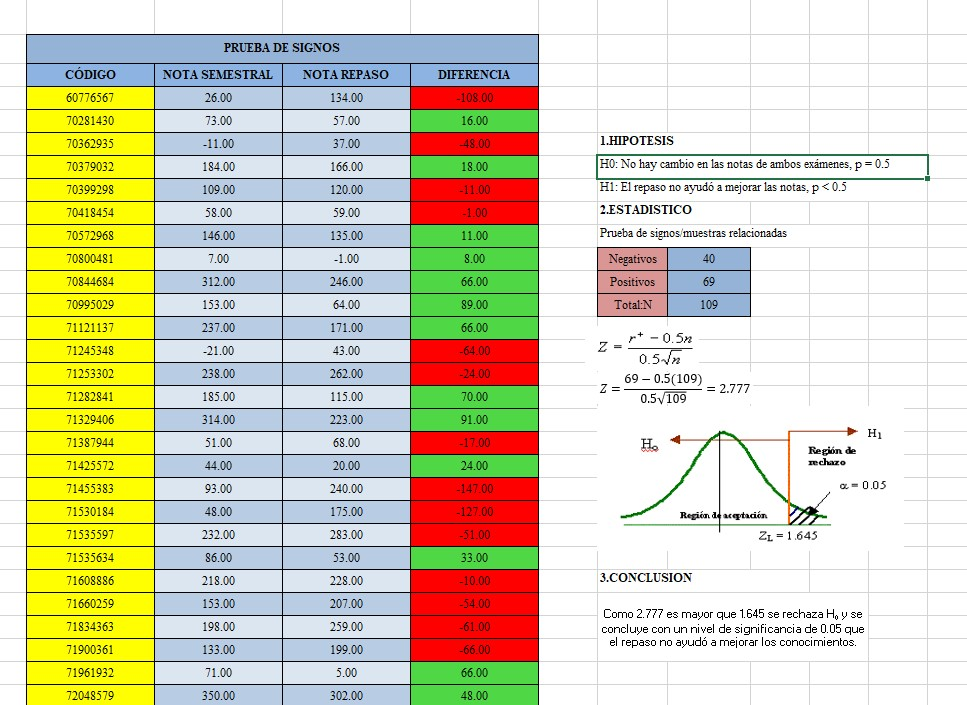
\includegraphics[width=0.8\textwidth]{cap/images/signos/signos.jpg}
\end{frame}


\begin{frame}
    \frametitle{Test de Wilcoxon}
    Si bien, el test de signos puede cumplir la misma funcion que el de
    \textbf{Wilcoxon}, este ultimo tiene mayor potencia al momento de
    detectar diferencia de medias.
  
\end{frame}

\begin{frame}
    \frametitle{Prueba de Wilcoxon}
    Se realiza una prueba de Wilcoxon para 2 muestras
    \textbf{relacionadas} 
    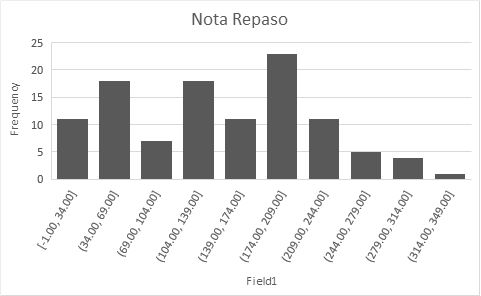
\includegraphics[width=1\textwidth]{cap/images/wilcoxon/repaso.jpg}
\end{frame}

\begin{frame}
    \frametitle{Prueba de Wilcoxon}
    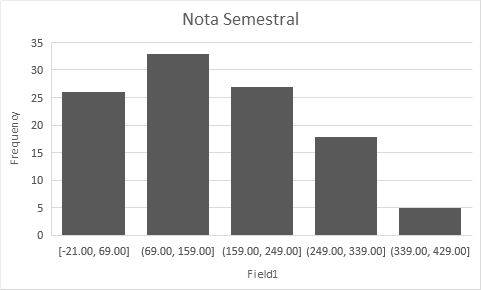
\includegraphics[width=1\textwidth]{cap/images/wilcoxon/semestral.jpg}
\end{frame}

\begin{frame}

    \frametitle{Prueba de Wilcoxon}

    \[H_0: \textrm{Las distribuciones son semejantes}\]
    
    \[H_1: \textrm{Las distribuciones se encuentran desplazadas}\]

    Dado que el estadistico de prueba: \[ Z = 2.991 \] es mayor al 
    \[Z_crit = 1.645\] se rechaza la hipotesis nula, por lo que se no
    se puede afirmar que ambas muestras sean identicas.

    \textbf{El repaso no ayudó a mejorar los conocimientos}
\end{frame}

\begin{frame}
    \frametitle{Prueba de Wilcoxon}
    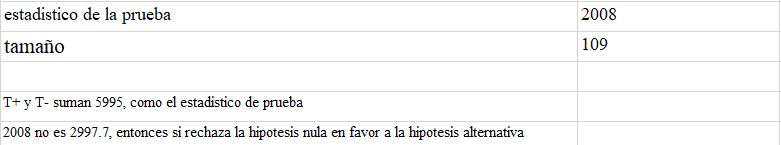
\includegraphics[width=1\textwidth]{cap/images/wilcoxon/resultados.jpg}
\end{frame}


%---------------------------------------------------------


\section{Conclusiones}

\begin{frame}
  \frametitle{Conclusiones}
  \begin{itemize}
    \item El ciclo de repaso no ha mejorado las notas de los estudiantes de la academia Trilce. Sin embargo 
    esto podría deberse a que el examen después de repaso fue más complicado que el examen antes de repaso, cosa que no 
    tenemos por seguro. 
    \item La distribución de estudiantes de Villa el Salvador es diferente a la de los demás distritos como mínimo. 
    \item Las mujeres y hombres tienen un desempeño similar en el examen de repaso.
    \item Existe diferencia en el desempeño pre-pandemia y post-pandemia de los estudiantes de la academia Trilce.
  \end{itemize}
\end{frame}

\end{document}
